\documentclass{homework}
\usepackage{ctex, bm}
\usepackage{makecell}
\usepackage[ruled,vlined]{algorithm2e}
\usepackage{booktabs}
\usepackage{multirow}
\usepackage{siunitx}
\usepackage{graphicx}
\usepackage{amsmath}
% \usepackage{subcaption}
\usepackage{caption}
\newcommand{\bfx}{\mathbf{x}}
\newcommand{\bfg}{\mathbf{g}}
\newcommand{\bfH}{\mathbf{H}}
\newcommand{\bfd}{\mathbf{d}}
\author{李健宁}
\class{机器学习中的优化问题}
\date{\today}
\title{Homework 11}
% \address{Bayt El-Hikmah}

\graphicspath{{./media/}}

\begin{document} \maketitle

\question

\begin{sol}
把目标函数改写一下,
\begin{equation}
\min_{A u = 0} \left\| -\nabla f(x) - u \right\|_2 \Leftrightarrow \min_{A u = 0}
\frac{1}{2}\left\|u + \nabla f(x)\right\|_2^2 \label{1-1}
\end{equation}

引入等式约束$Au=0$的拉格朗日乘子$w$,根据一阶条件和可行性条件,有

    \[
    \frac{\partial \mathcal{L}}{\partial u} = u + \nabla f(x) + A^T w = 0
    \quad \Rightarrow \quad
    u + A^T w = -\nabla f(x).
    \]
    \[
    A u = 0.
    \]

这两式正是$v$所满足的条件,根据题目,$v$是该方程组的唯一解,因此$v$就是最优化问题(\ref{1-1})的最小值点。

对于$w$,同样改写目标函数,
\begin{equation*}
    \min\left\| \nabla f(x) + A^\top y \right\|_2 \Leftrightarrow   \min\frac{1}{2}\left\| \nabla f(x) + A^\top y \right\|_2^2,
\end{equation*}

设$y^*$是上述问题的解,根据一阶条件得$0 = -A(\nabla f(x) - A^\top y^*)$, 将$\nabla f(x) = -v - A^\top w $代入并利用$Av=0$,有
\begin{equation*}
    A(-v - A^\top w + A^\top y^*) = 0 \Leftrightarrow   AA^\top w =AA^\top y^*.
\end{equation*}

根据题目中描述,原方程组只有唯一解,因此只可能$w= y^*$。

\end{sol}

\question

\begin{sol}
    

为保证可行性,先随机生成一个 $x^0$,然后令$b=A x^0, $这样 $x^0$ 即为一个可行初始点。
梯度和Hessian矩阵
$$
 \nabla f(x)=\frac{e^x}{\sum_j e^{x_j}}=:p(x),
\quad \nabla^2 f(x)=\mathrm{diag}(p(x))-p(x)p(x)^T.
$$

\subsection*{投影梯度法}

投影矩阵$ P=I-A^T(AA^T)^{-1}A,$迭代方向$ d_k=-P\nabla f(x_k),$

利用Backtracing线搜索确定步长,参数 $\alpha = 0.3, \beta = 0.5$,停止标准
$$ f(x_k+t d_k)\le f(x_k)+\alpha t\nabla f(x_k)^T d_k,$$
更新$$ x_{k+1}=x_k+t d_k.$$

算法停止标准$| x_{k+1}-x_k|\le \epsilon = 10^{-4}.$

\subsection*{带等式约束的Damped Newton法}

构造 KKT 条件
$$
 \begin{pmatrix} H_k & A^T \\ A & 0 \end{pmatrix}
 \begin{pmatrix} \Delta x \\ \Delta\lambda \end{pmatrix}
 = -\begin{pmatrix} \nabla f(x_k) \\ 0 \end{pmatrix},
$$
其中 $H_k=\nabla^2 f(x_k)$。解得 $\Delta x$ 后,同样用 Backtracing线搜索确定步长,参数同上,更新
$$ x_{k+1}=x_k+t\Delta x.$$
$$\lambda(x) = (\Delta x \nabla^2f(x) \Delta x)^{\frac12},$$
算法停止标准$\lambda^2/2\le \epsilon = 10^{-4}.$

\subsection*{对偶方法}先求对偶问题。
\begin{equation}\label{2-1}
\begin{aligned}
    \mathcal L(x,\nu) &=  f(x) + \nu^T(Ax-b) \\
    \frac{\partial \mathcal L}{\partial x_i}  &= \frac{e^{x_i}}{e^{f(x)}} + [\nu^TA]_i = 0 
    \end{aligned}
\end{equation}
\begin{equation}
    \begin{aligned}
    \Rightarrow \hat x_i &= f(\hat x) + \log(-[\nu^TA]_i) \\
    \Rightarrow g(\nu) &= \inf_{x\in\mathbb{R}^n}\,\mathcal L(x,\nu) \\
    &= \mathcal L(\hat x,\nu) \\
    &= \log \Sigma_i (-[\nu^TA]_ie^{f(\hat x)}) + \nu^T(A\hat x -b) \\
    & = f(\hat x) + \log\Sigma_i(-[\nu^TA]_i) + \nu^T(A\hat x -b)
\end{aligned}   
\end{equation}
根据(\ref{2-1}),有$\Sigma_i -[\nu^TA]_i = 1$和$-[\nu^TA]_i > 0$。代入有
\begin{equation}
    \begin{aligned}
        f(\hat x) + \nu^TA\hat x & = f(\hat x) + \nu^TA(f(\hat x) + \log (-\nu^TA)) \\&= f(\hat x) + \Sigma_i [\nu^TA]_i f(\hat x) + \Sigma_i[\nu^TA]_i\log(-[\nu^TA]_i) \\&= \Sigma_i[\nu^TA]_i\log(-[\nu^TA]_i) \\
        \log\Sigma_i(-[\nu^TA]_i) &= \log 1 = 0
    \end{aligned}
\end{equation}

因此
\[
g(\nu) = \Sigma_i[\nu^TA]_i\log(-[\nu^TA]_i) - \nu^Tb
\]

对偶问题
\[
\max_{\nu\in\mathbb{R}^p}\;g(\nu)
\;=\;
\max_{\nu}\;
\Sigma_i[\nu^TA]_i\log(-[\nu^TA]_i) - \nu^Tb \quad\;\text{s.t.} \;\Sigma_i s_i = 1, s >0
\]
其中$s_i = -[\nu^TA]_i$,
对对偶问题使用Damped Newton法求解,参数设置同上。

\subsection*{性能对比}

运行三种算法若干迭代,记录每次迭代的目标值 $f(x_k)$,并用 Newton 方法的高精度解近似最优值 $f^*$,绘制$ \log\bigl(f(x_k)-f^*\bigr)
$关于迭代次数的曲线,比较收敛速度,如图\ref{fig:2-1}。
\begin{figure}
    \centering
    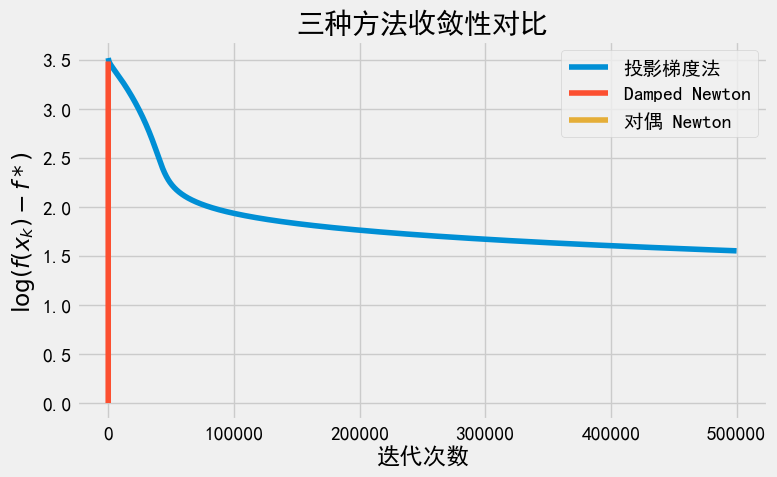
\includegraphics[width=0.5\linewidth]{image.png}
    \caption{三种方法收敛性对比}
    \label{fig:2-1}
\end{figure}

可以看到投影梯度法收敛非常慢。

\end{sol}

\question

\begin{sol}
    两个目标函数分别是
    \[
    \min_x \frac 12 \|x\|_2^2+\lambda \|Ax-b\|_1
    \]
    和
    \[
    \min_x \frac 12 \|x\|_2^2+\gamma\|Ax-b\|_2^2.
    \]
显式解是$x^* = A^T(AA^T)^{-1}b$,所以$f^* = f(x^*)$。参数选取上,$\lambda = \gamma = 10^{-3}$,$\log (f(x_k) - f^*)$与迭代次数的关系如图\ref{fig:3-1}.
\begin{figure}.
    \centering
    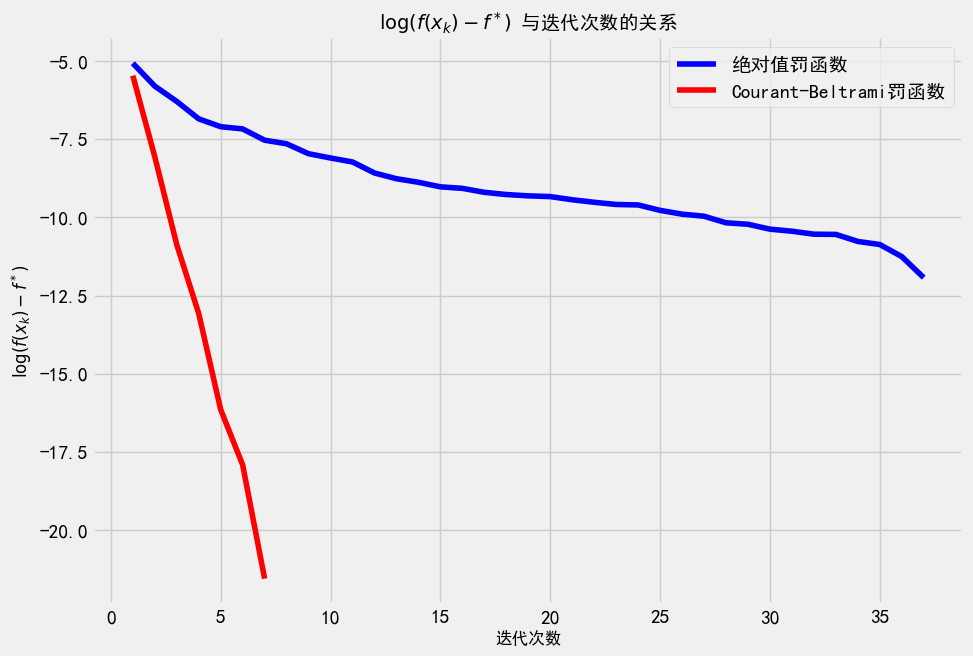
\includegraphics[width=0.5\linewidth]{image2.png}
    \caption{$\log (f(x_k) - f^*)$与迭代次数的关系.}
    \label{fig:3-1}
\end{figure}
\end{sol}


% citations
% \bibliographystyle{plain}
% \bibliography{citations}

\end{document}
